\documentclass[11pt,a4paper]{article}

% Compile from the repository root with:
% pdflatex reports/customer_value_project_report.tex
% The figures are loaded from reports/figures/.
\usepackage[utf8]{inputenc}
\usepackage[T1]{fontenc}
\usepackage{lmodern}
\usepackage[a4paper,margin=0.82in,headheight=22pt]{geometry}
\usepackage{xcolor}
\usepackage{graphicx}
\usepackage{booktabs}
\usepackage{tabularx}
\usepackage{array}
\usepackage{enumitem}
\usepackage{float}
\usepackage{caption}
\usepackage{titlesec}
\usepackage{fancyhdr}
\usepackage{hyperref}
\usepackage{microtype}
\usepackage{parskip}

\definecolor{Navy}{HTML}{17365D}
\definecolor{Blue}{HTML}{315FBD}
\definecolor{LightBlue}{HTML}{EAF1FB}
\definecolor{Ink}{HTML}{263445}
\definecolor{Muted}{HTML}{627386}
\definecolor{Rule}{HTML}{D9E2EF}

\hypersetup{
  colorlinks=true,
  linkcolor=Navy,
  urlcolor=Blue,
  citecolor=Navy,
  pdftitle={Customer Lifetime Value Prediction Engine},
  pdfauthor={Shurya Singhal, Arnav Rai, Ishi Agarwal, Vasvi Sood}
}
\graphicspath{{reports/figures/}{figures/}}
\setlength{\parindent}{0pt}
\setlength{\parskip}{5pt}
\setlist[itemize]{leftmargin=1.35em,itemsep=3pt,topsep=4pt}
\renewcommand{\arraystretch}{1.18}
\titleformat{\section}{\Large\bfseries\color{Navy}}{\thesection}{0.65em}{}
\titleformat{\subsection}{\large\bfseries\color{Blue}}{\thesubsection}{0.65em}{}
\captionsetup{font=small,labelfont={bf,color=Navy},textfont={color=Muted}}

\pagestyle{fancy}
\fancyhf{}
\fancyhead[L]{\small\color{Muted}Customer Value Prediction Engine}
\fancyhead[R]{\small\color{Muted}Project Report}
\fancyfoot[C]{\small\color{Muted}\thepage}
\renewcommand{\headrulewidth}{0.4pt}
\renewcommand{\headrule}{\hbox to\headwidth{\color{Rule}\leaders\hrule height \headrulewidth\hfill}}

\newcolumntype{Y}{>{\raggedright\arraybackslash}X}
\newcommand{\GBP}{\pounds}
\newcommand{\metric}[2]{\textbf{#1} & #2\\}

\begin{document}

% -----------------------------------------------------------------------------
% Cover
% -----------------------------------------------------------------------------
\begin{titlepage}
  \thispagestyle{empty}
  \vspace*{1.15in}
  {\color{Blue}\rule{\textwidth}{2pt}}\\[0.35in]
  {\Large\color{Blue}\bfseries DATA SCIENCE PROJECT REPORT}\\[0.25in]
  {\Huge\color{Navy}\bfseries Customer Lifetime Value\\[0.08in]
   Prediction Engine}\\[0.25in]
  {\Large\color{Muted}Six-month customer revenue forecasting and retention prioritization}\\[0.55in]

  \begin{tabularx}{\textwidth}{@{}>{\bfseries\color{Navy}}l Y@{}}
    Project & Customer Lifetime Value Prediction Engine\\
    Dataset & UCI Online Retail II\\
    Forecast horizon & Six months\\
    Scoring cutoff & 1 March 2011\\
  \end{tabularx}

  \vfill
  {\large\bfseries\color{Navy}Project team}\\[0.12in]
  \begin{tabularx}{\textwidth}{@{}Y r@{}}
    Shurya Singhal & 590023883\\
    Arnav Rai & 590027562\\
    Ishi Agarwal & 590025685\\
    Vasvi Sood & 590027632\\
  \end{tabularx}
  \vspace{0.35in}
  {\color{Blue}\rule{\textwidth}{2pt}}
\end{titlepage}

\pagenumbering{roman}
\tableofcontents
\clearpage
\pagenumbering{arabic}

% -----------------------------------------------------------------------------
\section{Executive summary}

This project turns historical online retail transactions into customer-level
forecasts and retention priorities. For each customer, it estimates revenue
over the next six months and estimates the probability of no purchase in the
first 90 days after the scoring date. These two estimates support customer
prioritization; they do not guarantee future spending or campaign response.

The analysis uses a chronological evaluation: customer features are calculated
from transactions before 1 March 2011, and forecasts are compared with actual
revenue from March through August 2011. Of the three revenue methods compared,
BG/NBD + Gamma-Gamma delivered the lowest holdout error (MAE \GBP 558.32) and
the highest revenue capture in its top predicted quintile (77.8\%).

The scored portfolio contains 4,537 customers. The Champions group contains
887 customers and 71.5\% of predicted portfolio revenue. The model and
segments are best treated as decision support: the data is historical, covers
one UK retailer, and records revenue rather than profit.

\subsection*{Key results}
\begin{center}
\begin{tabular}{@{}lr@{}}
\toprule
\metric{Identified customers in cleaned dataset}{5,878}
\metric{Customers scored at the March 2011 cutoff}{4,537}
\metric{Best holdout MAE}{\GBP 558.32}
\metric{Best holdout $R^2$}{0.782}
\metric{Revenue captured in top predicted 20\%}{77.8\%}
\bottomrule
\end{tabular}
\end{center}

\section{Business problem and objectives}

Marketing teams have limited time and budget for retention outreach. A useful
starting point is to identify which customers are expected to generate more
revenue and which may become inactive soon. The project addresses this by:
\begin{itemize}
  \item estimating each customer's revenue for a defined six-month horizon;
  \item estimating short-term purchase inactivity risk;
  \item grouping customers into interpretable value-and-risk segments;
  \item comparing forecast models on a later, held-out time period; and
  \item presenting the results through reports and an interactive dashboard.
\end{itemize}

In this report, ``customer lifetime value'' is operationalized as a
\textbf{six-month revenue forecast}. It is not a prediction of total revenue
over the customer's entire relationship with the retailer, and revenue is not
the same as profit.

\section{Dataset and preparation}

The source is the UCI Online Retail II dataset, containing 1,067,371 transaction
lines from a UK non-store retailer between December 2009 and December 2011.
The dataset is available under CC BY 4.0. The source workbook is loaded from
\texttt{data/raw/online\_retail\_II.xlsx} and is not committed to Git.

\begin{table}[H]
\centering
\caption{Transaction cleaning summary}
\label{tab:cleaning}
\begin{tabularx}{0.9\textwidth}{@{}Y r@{}}
\toprule
\textbf{Cleaning step} & \textbf{Rows}\\
\midrule
Raw transaction lines (input) & 1,067,371\\
Rows without customer ID & 243,007\\
Exact duplicate rows & 26,479\\
Cancelled invoices & 18,390\\
Non-positive prices & 70\\
\midrule
Positive purchase lines retained & 779,425\\
\bottomrule
\end{tabularx}
\end{table}

Customer-linked negative-quantity rows are saved separately and excluded from
purchase revenue modeling. The cleaning process also writes an audit file so
row removals can be reviewed. After cleaning, 5,878 distinct customers are
present in the transaction history.

\subsection{Exploratory analysis}

The figures below summarize the cleaned data. They are descriptive patterns;
they do not explain why customers purchased or establish causal effects.

\begin{figure}[H]
\centering
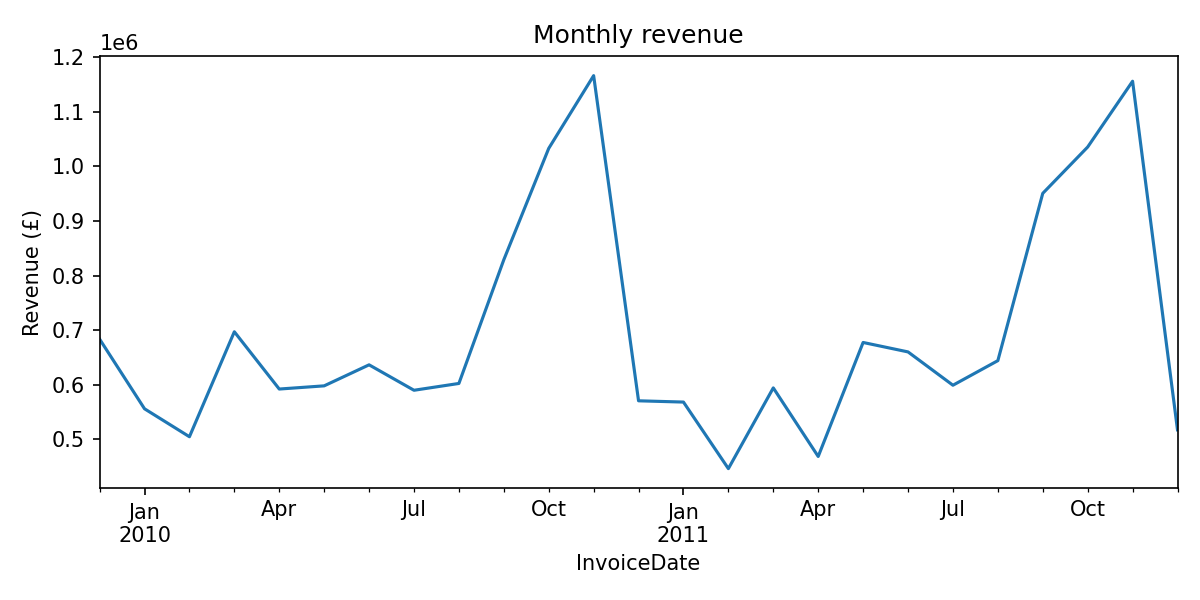
\includegraphics[width=0.82\textwidth]{monthly_revenue.png}
\caption{Monthly revenue across the transaction history. Revenue peaks are
descriptive and may reflect seasonality, business activity, or other factors.}
\label{fig:monthly}
\end{figure}

\begin{figure}[H]
\centering
\begin{minipage}[t]{0.48\textwidth}
  \centering
  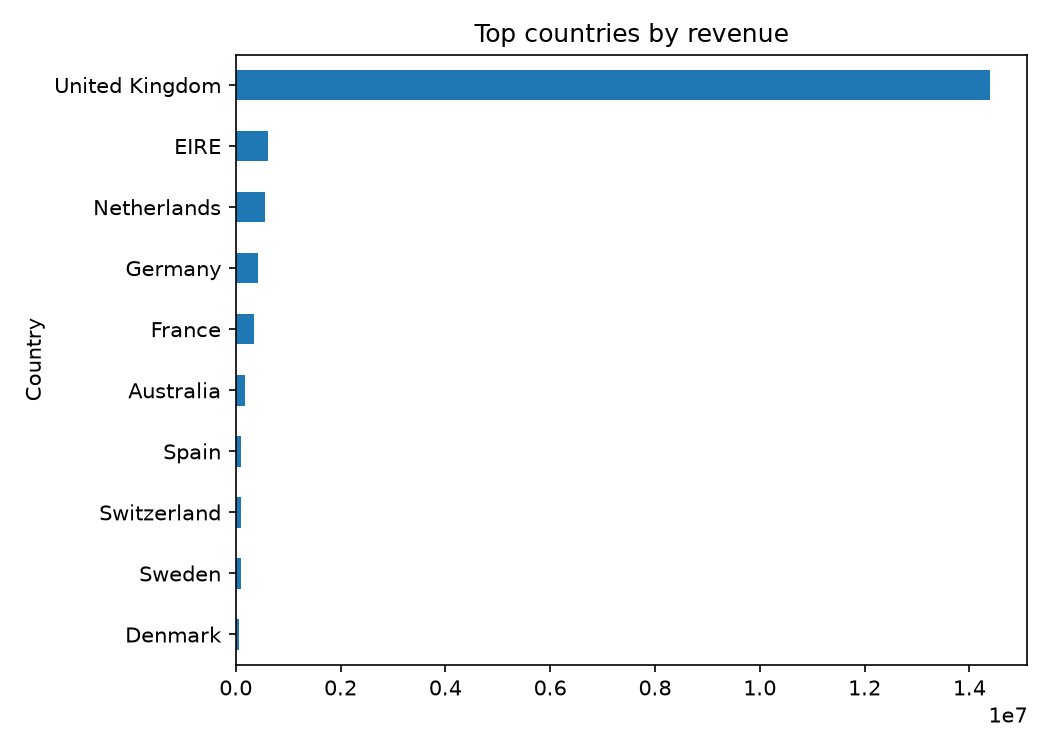
\includegraphics[width=\textwidth]{top_countries.png}
  \caption{Top countries by cleaned revenue. The UK contributes 82.8\% of
  cleaned revenue.}
  \label{fig:countries}
\end{minipage}\hfill
\begin{minipage}[t]{0.48\textwidth}
  \centering
  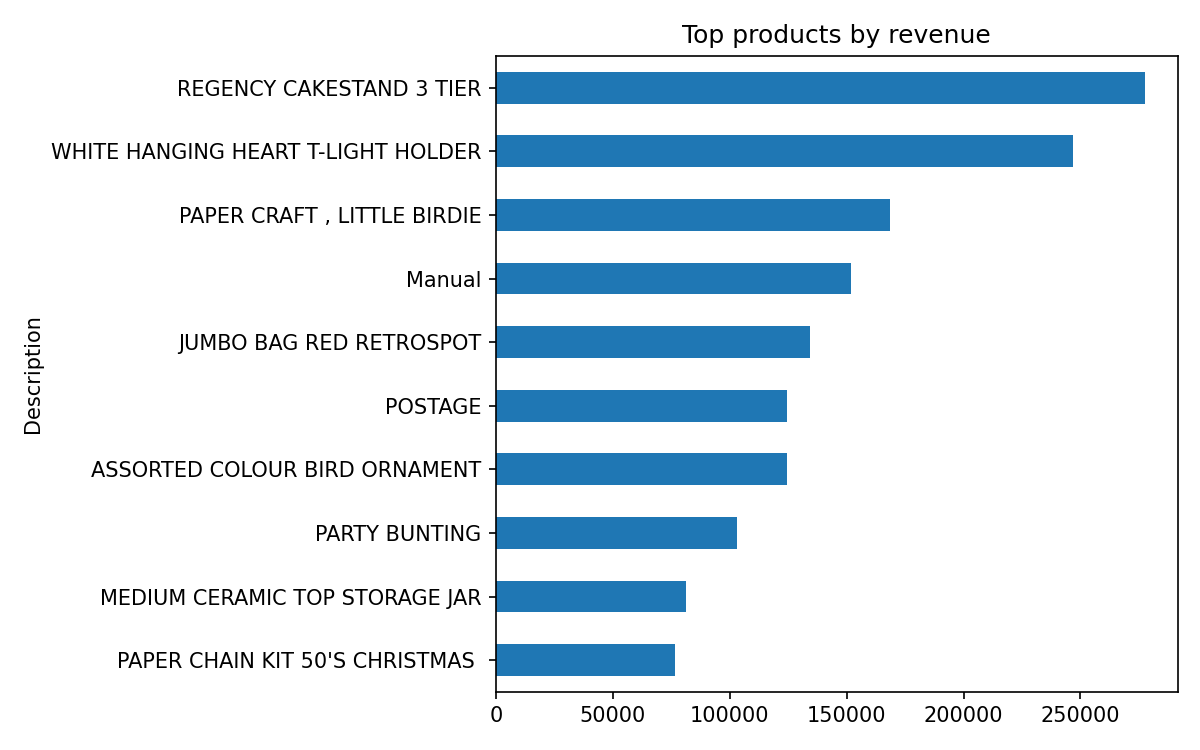
\includegraphics[width=\textwidth]{top_products.png}
  \caption{Ten highest-revenue products. Together they contribute 8.6\% of
  cleaned sales.}
  \label{fig:products}
\end{minipage}
\end{figure}

\begin{figure}[H]
\centering
\begin{minipage}[t]{0.48\textwidth}
  \centering
  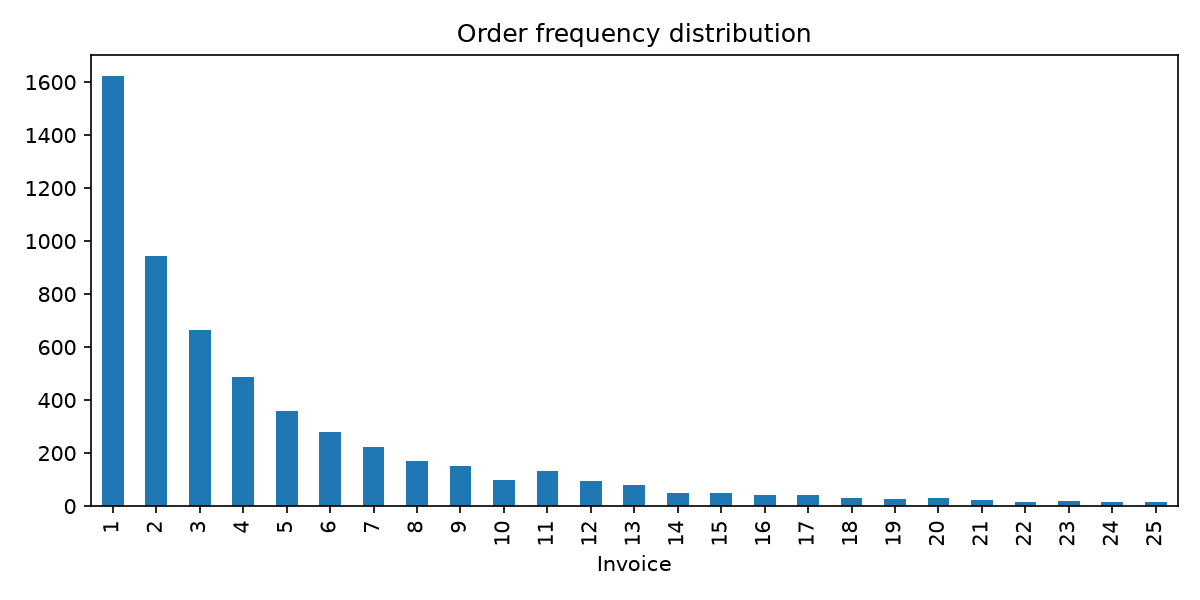
\includegraphics[width=\textwidth]{order_frequency.png}
  \caption{Customer order frequency. In total, 72.4\% of identified customers
  placed at least two orders.}
  \label{fig:frequency}
\end{minipage}\hfill
\begin{minipage}[t]{0.48\textwidth}
  \centering
  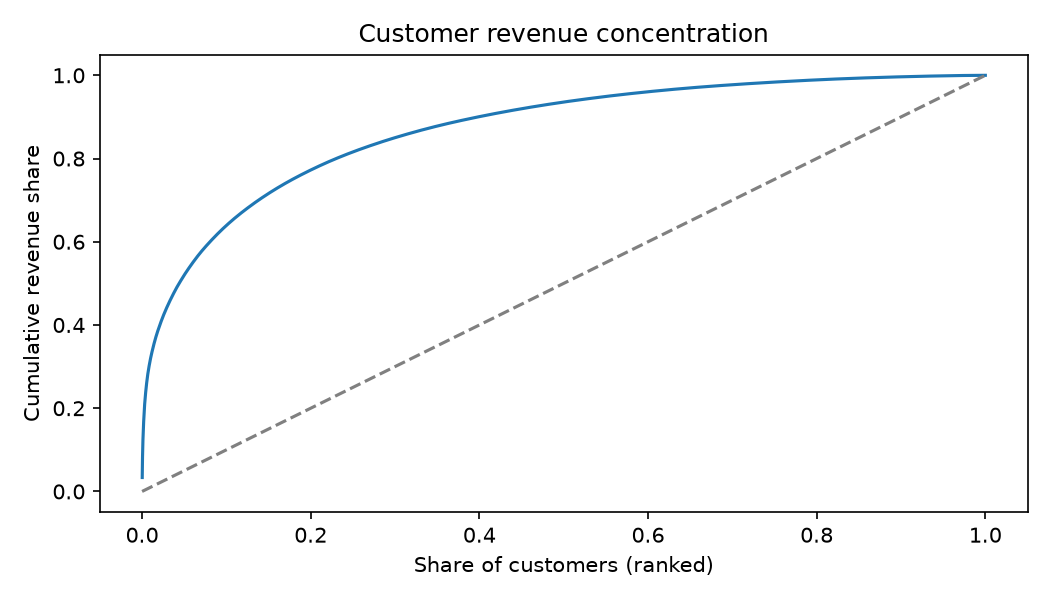
\includegraphics[width=\textwidth]{pareto_curve.png}
  \caption{Cumulative customer revenue concentration. The top fifth of
  customers account for 77.2\% of cleaned revenue.}
  \label{fig:pareto}
\end{minipage}
\end{figure}

\section{Feature engineering and time-based design}

The final scoring cutoff is 1 March 2011. All customer features use transactions
strictly before the cutoff. The six-month revenue target uses transactions from
the cutoff through 31 August 2011. Inactivity is defined as no purchase during
the first 90 days after the cutoff. Future target rows are kept separate from
the features to prevent temporal leakage.

\begin{table}[H]
\centering
\caption{Customer features used by the modeling pipeline}
\label{tab:features}
\begin{tabularx}{\textwidth}{@{}>{\bfseries}l Y@{}}
\toprule
Feature & Meaning\\
\midrule
Recency & Days since the customer's last purchase before cutoff\\
Frequency & Number of distinct invoices before cutoff\\
Monetary & Total historical purchase revenue before cutoff\\
Tenure & Days between first and last observed purchase\\
Average order value & Historical revenue divided by distinct invoices\\
Order intervals & Mean and standard deviation of days between purchases\\
Product breadth & Number of distinct products purchased\\
Return rate & Historical return invoices relative to purchase and return invoices\\
Q4 order share & Share of invoices placed in the fourth calendar quarter\\
\bottomrule
\end{tabularx}
\end{table}

To evaluate forecasts chronologically, earlier monthly snapshots are used to
train the models, and an out-of-time snapshot is used for validation. Tree
regularization is selected on an earlier snapshot than the final evaluation.
Thus the model comparison reflects a later holdout rather than a random split
of transaction rows.

\section{Modeling approach}

\subsection{Six-month revenue forecast}
Three approaches are compared:
\begin{itemize}
  \item \textbf{Historical average:} spreads observed customer revenue over the
  observed history to form a transparent baseline.
  \item \textbf{BG/NBD + Gamma-Gamma:} estimates expected purchase frequency and
  expected order value, then combines them into a six-month revenue forecast.
  \item \textbf{Gradient boosting:} learns nonlinear relationships between the
  engineered customer features and future revenue.
\end{itemize}

\subsection{Inactivity risk and customer groups}

A random forest classifier estimates whether a customer makes no purchase in
the first 90 days after the cutoff. The value forecast and risk estimate are
then combined into five rules-based groups: Champions, Loyal, Potential,
At-Risk, and Hibernating. These labels support prioritization; they are not
causal treatment recommendations.

\section{Results}

\subsection{Revenue forecast comparison}

Table~\ref{tab:model-results} reports the chronological holdout metrics. Lower
MAE and RMSE indicate smaller forecast errors. Higher $R^2$ indicates a better
fit to variation in holdout revenue. ``Top 20\% capture'' measures how much
actual holdout revenue falls among customers ranked in the highest predicted
fifth.

\begin{table}[H]
\centering
\caption{Out-of-time model comparison (six-month revenue, GBP)}
\label{tab:model-results}
\begin{tabular}{@{}lrrrr@{}}
\toprule
\textbf{Model} & \textbf{MAE} & \textbf{RMSE} & \textbf{$R^2$} & \textbf{Top 20\% capture}\\
\midrule
Historical average & \GBP 573.32 & \GBP 2,004.53 & 0.683 & 76.5\%\\
BG/NBD + Gamma-Gamma & \textbf{\GBP 558.32} & \textbf{\GBP 1,661.35} & \textbf{0.782} & \textbf{77.8\%}\\
Gradient boosting & \GBP 1,241.12 & \GBP 3,017.85 & 0.282 & 76.4\%\\
\bottomrule
\end{tabular}
\end{table}

BG/NBD + Gamma-Gamma has the lowest MAE and RMSE and the highest top-quintile
revenue capture in this holdout. The top predicted decile averages 6.39 times
the validation-wide mean revenue. This describes ranking performance on this
historical holdout and should not be read as a guaranteed result on new data.

\begin{figure}[H]
\centering
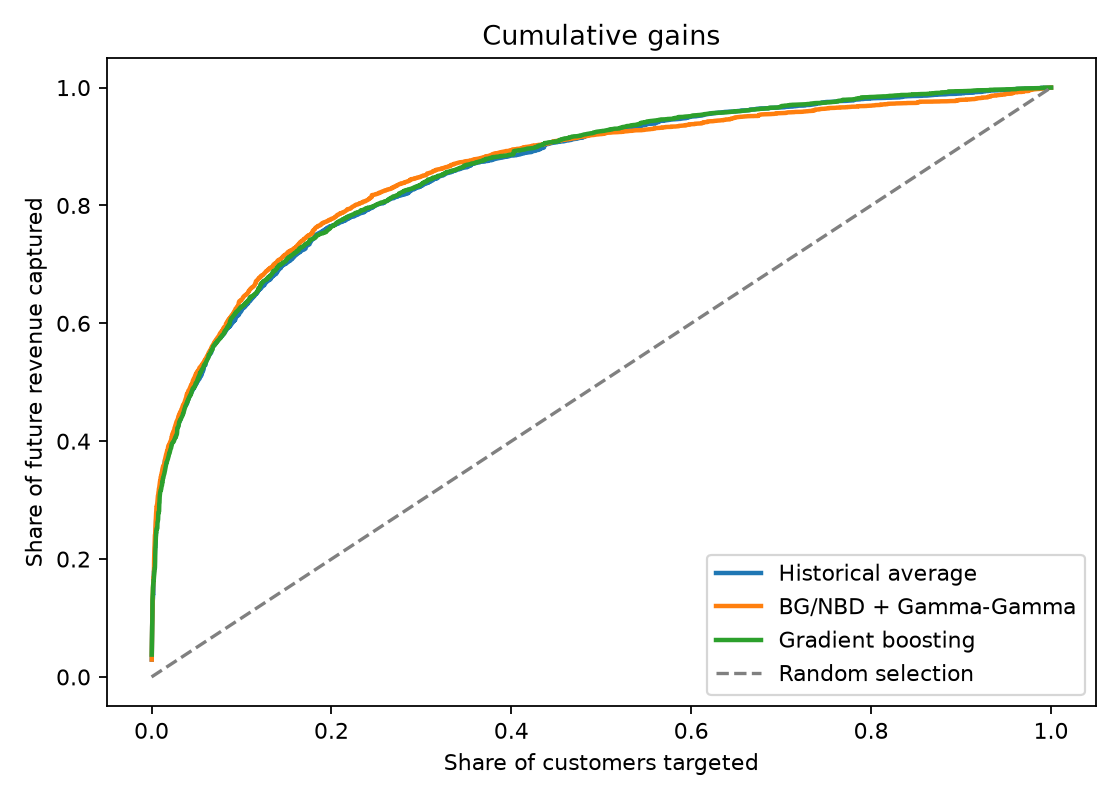
\includegraphics[width=0.76\textwidth]{cumulative_gains.png}
\caption{Cumulative gains by model. Curves show the share of actual holdout
revenue captured as customers are selected in descending forecast order.}
\label{fig:gains}
\end{figure}

\subsection{Feature importance}

Permutation importance for the gradient-boosting model identifies monetary
history as its strongest positive driver of validation performance, followed
by purchase frequency, tenure, and product breadth. This measures model
reliance on features, not causal influence on customer spending.

\begin{table}[H]
\centering
\caption{Leading gradient-boosting permutation-importance results}
\label{tab:importance}
\begin{tabular}{@{}lr@{}}
\toprule
\textbf{Feature} & \textbf{Mean importance}\\
\midrule
Monetary history & 875.64\\
Purchase frequency & 344.05\\
Tenure & 143.19\\
Distinct products & 138.27\\
Q4 order share & 101.58\\
Mean order interval & 84.85\\
\bottomrule
\end{tabular}
\end{table}

\subsection{Customer segment profile}

Table~\ref{tab:segments} summarizes the 4,537 customers scored at the cutoff.
Champions account for the largest share of predicted portfolio revenue.
At-Risk is a small group with comparatively high average inactivity risk.

\begin{table}[H]
\centering
\caption{Customer segment summary at the scoring cutoff}
\label{tab:segments}
\begin{tabular}{@{}lrrrr@{}}
\toprule
\textbf{Segment} & \textbf{Customers} & \textbf{Forecast revenue} & \textbf{Avg. risk} & \textbf{Revenue share}\\
\midrule
Champions & 887 & \GBP 3,023,500 & 17.3\% & 71.5\%\\
Loyal & 1,192 & \GBP 735,130 & 31.3\% & 17.4\%\\
Potential & 1,672 & \GBP 287,741 & 55.2\% & 6.8\%\\
At-Risk & 21 & \GBP 84,143 & 64.7\% & 2.0\%\\
Hibernating & 765 & \GBP 100,385 & 78.1\% & 2.4\%\\
\bottomrule
\end{tabular}
\end{table}

\subsection{Illustrative planning scenario}

An optional scenario selects Champions plus At-Risk (908 customers) and assumes
a 30\% contribution margin, 10\% incremental retained revenue, and \GBP 1
contact cost per selected customer. Under those assumptions, estimated net
benefit is \GBP 92,321. This is a sensitivity scenario only: retention uplift
and margin are not measured by this project, and no campaign experiment was
conducted. It should not be treated as a causal ROI estimate or budget
commitment.

\section{Application and reproducibility}

The repository includes a Streamlit dashboard for reviewing the portfolio,
exploring segments, searching customer IDs, viewing model results, and scoring
an uploaded transaction file. The pipeline writes cleaned data and an audit
to \texttt{data/processed/}, model outputs to \texttt{reports/}, and figures to
\texttt{reports/figures/}.

On Windows, install Python 3.11 and run \texttt{run\_project.bat} from the
project folder. The launcher creates a virtual environment, installs the
requirements, builds outputs when needed, and starts the dashboard. To rebuild
the pipeline outputs, run \texttt{run\_project.ps1 -Rebuild}. The manual
pipeline entry point is \texttt{python run\_pipeline.py}.

\section{Limitations and recommendations}

\begin{itemize}
  \item The dataset describes one UK retailer and ends in 2011; present-day
  behavior may differ.
  \item Transaction price is revenue, not contribution margin or profit.
  \item Customer demographics, marketing exposure, and campaign responses are
  not available in the source data.
  \item The 90-day inactivity definition and six-month revenue horizon are
  operational choices; alternative definitions may produce different groups.
  \item The ROI scenario is assumption-based. A controlled holdout experiment
  should measure incremental response, margin, and contact cost before scaling.
  \item Before operational use, validate forecasts on recent transactions and
  monitor performance as customer behavior changes.
\end{itemize}

\section{Conclusion}

The project provides a reproducible workflow for transforming transaction
history into customer value forecasts, inactivity-risk estimates, and
interpretable retention groups. On the historical chronological holdout,
BG/NBD + Gamma-Gamma was the strongest revenue forecasting method among those
compared. The results support prioritization and further testing; current
data and controlled experiments are required before using them to make
production or budget decisions.

\section*{References}
\addcontentsline{toc}{section}{References}
\begin{enumerate}[label={[\arabic*]},leftmargin=2em]
  \item Chen, D. (2012). \emph{Online Retail II}. UCI Machine Learning
  Repository. \href{https://doi.org/10.24432/C5CG6D}{doi:10.24432/C5CG6D}.
  Dataset license: CC BY 4.0.
  \item UCI Machine Learning Repository. \emph{Online Retail II dataset}.
  \href{https://archive.ics.uci.edu/dataset/502/online+retail+ii}{Dataset page}.
\end{enumerate}

\end{document}
